\documentclass[aspectratio=169]{beamer}
% Add slides directory to search path for Dartmouth theme
\makeatletter
\def\input@path{{../}}
\makeatother
\usetheme{Dartmouth}

% Packages
\usepackage{fontspec}
\usepackage{listings}
\usepackage{xcolor}
\usepackage{tcolorbox}
\usepackage{booktabs}
\usepackage{hyperref}
\usepackage{tikz}
\usetikzlibrary{shapes,arrows,positioning,calc,decorations.pathreplacing}

% Font settings
\setmonofont{Courier New}

% Code listing settings
\lstset{
    language=Python,
    basicstyle=\ttfamily\small,
    keywordstyle=\color{blue},
    commentstyle=\color{gray},
    stringstyle=\color{red},
    showstringspaces=false,
    breaklines=true,
    frame=single,
    numbers=left,
    numberstyle=\tiny\color{gray}
}

% Custom colors
\definecolor{thinkbox}{RGB}{255,245,220}
\definecolor{discussbox}{RGB}{230,240,255}

% Custom boxes
\newtcolorbox{thinkaboutit}{
    colback=thinkbox,
    colframe=orange,
    title=💭 Think about it!,
    fonttitle=\bfseries
}

\newtcolorbox{discussion}{
    colback=discussbox,
    colframe=blue,
    title=💬 Discussion,
    fonttitle=\bfseries
}

% Title page information
\title{Lecture 3: ELIZA Implementation}
\subtitle{The ELIZA Effect \& Your First Assignment 🎭}
\author{PSYC 51.07: Models of Language and Communication}
\institute{Dr. Jeremy R. Manning}
\date{Week 1 - Day 3}

\begin{document}

% Title slide
\begin{frame}[shrink=10]
\titlepage
\end{frame}

% Table of contents
\begin{frame}[shrink=5]{Today's Journey 🗺️}
\tableofcontents
\end{frame}

\section{Recap: Pattern Matching Fundamentals}

\begin{frame}{Last Time... 🔄}
\small
\begin{block}{Key Concepts from Lecture 2}
\begin{itemize}\setlength{\itemsep}{0pt}
    \item String manipulation and replacement
    \item Regular expressions for flexible patterns
    \item Capture groups for extracting information
    \item Pre and post substitutions
    \item ELIZA's basic architecture
\end{itemize}
\end{block}

\vspace{0.3cm}

\begin{discussion}
Today we'll complete the ELIZA implementation and explore its psychological impact!
\end{discussion}
\end{frame}

\section{Complete ELIZA Architecture}

\begin{frame}[fragile]{ELIZA Algorithm: Complete Version 🔧}
\begin{lstlisting}[basicstyle=\ttfamily\tiny]
def eliza_respond(user_input, rules):
    # 1. Pre-substitutions (normalize input)
    for old, new in PRE_SUBS.items():
        user_input = user_input.replace(old, new)

    # 2. Find all matching patterns
    matches = []
    for rule in rules:
        match = re.search(rule['pattern'], user_input)
        if match:
            matches.append((rule, match))

    # 3. Choose highest-ranked match
    if matches:
        best_rule, best_match = max(matches, key=lambda x: x[0]['rank'])

        # 4. Decompose - extract captured groups
        captured = best_match.groups()

        # 5. Reassemble - fill template with captures
        response = random.choice(best_rule['responses'])
        for i, group in enumerate(captured):
            response = response.replace(f'{{{i+1}}}', group)

        # 6. Post-substitutions (fix grammar)
        for old, new in POST_SUBS.items():
            response = response.replace(old, new)

        return response
    else:
        return random.choice(DEFAULT_RESPONSES)
\end{lstlisting}
\end{frame}

\begin{frame}[fragile]{Synonym Substitutions 📝}
\begin{block}{The Problem}
Users express the same idea in different ways:
\begin{itemize}\setlength{\itemsep}{0pt}
    \item "I am sad" vs "I am unhappy" vs "I am depressed"
    \item "My family" vs "My relatives" vs "My kin"
\end{itemize}
\end{block}

\vspace{0.3cm}

\textbf{ELIZA's solution: Synonym sets}

\begin{lstlisting}
SYNONYMS = {
    "family": ["family", "relatives", "kin", "folks"],
    "sad": ["sad", "unhappy", "depressed", "down", "blue"],
    "happy": ["happy", "glad", "joyful", "pleased", "content"],
    "remember": ["remember", "recall", "recollect"],
    "mother": ["mother", "mom", "mama", "mum"],
    "father": ["father", "dad", "papa", "pop"]
}
\end{lstlisting}

\vspace{0.3cm}

\textbf{Pattern:} \texttt{I am (sad|unhappy|depressed|down|blue)}
\end{frame}

\begin{frame}[fragile]{Building Patterns from Synonyms 🔨}
\begin{lstlisting}
def build_pattern(template, synonyms):
    """Convert template with synonym placeholders to regex"""
    for key, values in synonyms.items():
        placeholder = f"@{key}"
        if placeholder in template:
            options = "|".join(values)
            template = template.replace(placeholder, f"({options})")
    return template

# Example usage:
template = r"I am @sad"
pattern = build_pattern(template, SYNONYMS)
# Result: r"I am (sad|unhappy|depressed|down|blue)"

# Now can match ANY variant!
re.search(pattern, "I am depressed")  # ✓ Matches
re.search(pattern, "I am blue")       # ✓ Matches
re.search(pattern, "I am sad")        # ✓ Matches
\end{lstlisting}

\vspace{0.3cm}

\begin{thinkaboutit}
This makes ELIZA much more flexible without writing hundreds of separate patterns!
\end{thinkaboutit}
\end{frame}

\begin{frame}[fragile]{Memory and Context 🧠}
\begin{block}{Primitive State in ELIZA}
ELIZA can "remember" certain topics and bring them up later.
\end{block}

\vspace{0.3cm}

\begin{lstlisting}
class ElizaBot:
    def __init__(self):
        self.memory = []  # Store remembered topics

    def save_to_memory(self, topic):
        """Save a topic for later"""
        self.memory.append(topic)

    def recall_memory(self):
        """Retrieve a saved topic when needed"""
        if self.memory:
            topic = random.choice(self.memory)
            return f"Earlier you mentioned {topic}. Let's discuss that."
        return None

# Usage in a rule:
{
    "pattern": r"(.*) my (mother|father) (.*)",
    "rank": 100,
    "responses": [...],
    "save_to_memory": "{2}"  # Save "mother" or "father"
}
\end{lstlisting}
\end{frame}

\begin{frame}{Memory in Action 💡}
\begin{block}{Example Conversation with Memory}
\textbf{User:} I don't get along with my mother.\\
\textbf{ELIZA:} Tell me more about your mother. \textit{[Saves "mother" to memory]}

\textbf{User:} I like playing tennis.\\
\textbf{ELIZA:} That's interesting.

\textbf{User:} I don't know what to talk about.\\
\textbf{ELIZA:} Earlier you mentioned your mother. Let's discuss that.
\end{block}

\vspace{0.3cm}

\begin{thinkaboutit}
This simple memory creates the illusion of ELIZA "thinking about" what you said earlier! But it's just storing and randomly retrieving strings.
\end{thinkaboutit}
\end{frame}

\begin{frame}[shrink=5]{Complete ELIZA Flow with Memory 🔄}
\begin{center}
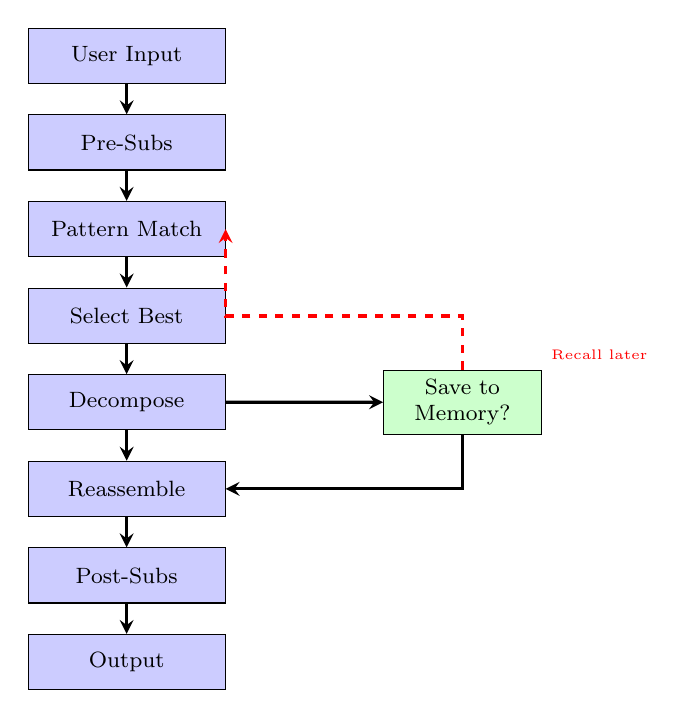
\begin{tikzpicture}[scale=0.85,
    node distance=1.1cm,
    box/.style={rectangle, draw, fill=blue!20, minimum width=2.5cm, minimum height=0.7cm, align=center, font=\footnotesize},
    membox/.style={rectangle, draw, fill=green!20, minimum width=2cm, minimum height=0.7cm, align=center, font=\footnotesize},
    arrow/.style={->, >=stealth, very thick}
]

% Main flow
\node[box] (input) {User Input};
\node[box, below of=input] (pre) {Pre-Subs};
\node[box, below of=pre] (match) {Pattern Match};
\node[box, below of=match] (rank) {Select Best};
\node[box, below of=rank] (decompose) {Decompose};

% Memory branch
\node[membox, right=2cm of decompose] (memory) {Save to\\Memory?};

\node[box, below of=decompose] (reassemble) {Reassemble};
\node[box, below of=reassemble] (post) {Post-Subs};
\node[box, below of=post] (output) {Output};

% Arrows - main flow
\draw[arrow] (input) -- (pre);
\draw[arrow] (pre) -- (match);
\draw[arrow] (match) -- (rank);
\draw[arrow] (rank) -- (decompose);
\draw[arrow] (decompose) -- (reassemble);
\draw[arrow] (reassemble) -- (post);
\draw[arrow] (post) -- (output);

% Memory arrows
\draw[arrow] (decompose) -- (memory);
\draw[arrow] (memory) |- (reassemble);

% Recall arrow
\draw[arrow, dashed, red] (memory.north) -- ++(0,0.8) -| (match.east);
\node[red, font=\tiny, above right] at (memory.north east) {Recall later};

\end{tikzpicture}
\end{center}
\end{frame}

\begin{frame}[fragile]{Default Responses 🎲}
\begin{block}{When No Pattern Matches}
ELIZA needs fallback responses when it can't find a matching pattern.
\end{block}

\vspace{0.3cm}

\begin{lstlisting}
DEFAULT_RESPONSES = [
    "I see.",
    "Tell me more.",
    "How does that make you feel?",
    "Why do you say that?",
    "Can you elaborate on that?",
    "What does that suggest to you?",
    "I'm not sure I understand. Can you rephrase?",
    "Interesting. Please continue.",
    "Go on..."
]

# Usage:
if no_pattern_matched:
    response = random.choice(DEFAULT_RESPONSES)
\end{lstlisting}

\vspace{0.3cm}

\begin{alertblock}{Clever Design}
These generic responses sound thoughtful but require zero understanding! They keep the conversation flowing.
\end{alertblock}
\end{frame}

\begin{frame}[fragile]{Quit Detection 🚪}
\begin{block}{Ending the Conversation}
ELIZA needs to recognize when the user wants to quit.
\end{block}

\vspace{0.3cm}

\begin{lstlisting}
QUIT_PATTERNS = [
    r"^quit$",
    r"^exit$",
    r"^bye$",
    r"^goodbye$",
    r"I have to go",
    r"I need to leave"
]

def should_quit(user_input):
    """Check if user wants to end conversation"""
    user_input = user_input.lower().strip()
    for pattern in QUIT_PATTERNS:
        if re.search(pattern, user_input):
            return True
    return False

# Quit responses
QUIT_RESPONSES = [
    "Goodbye. It was nice talking to you.",
    "That will be $200. See you next week!",
    "Take care!"
]
\end{lstlisting}
\end{frame}

\begin{frame}[fragile]{Main Conversation Loop 🔁}
\begin{lstlisting}[basicstyle=\ttfamily\tiny]
def main():
    """Main ELIZA conversation loop"""
    bot = ElizaBot()

    # Greeting
    print("ELIZA: Hello. I am ELIZA. What brings you here today?")
    print("(Type 'quit' to exit)\n")

    while True:
        # Get user input
        user_input = input("You: ").strip()

        # Check for quit
        if should_quit(user_input):
            print(f"ELIZA: {random.choice(QUIT_RESPONSES)}")
            break

        # Generate response
        response = bot.respond(user_input)
        print(f"ELIZA: {response}\n")

        # Occasionally recall memory (10% chance)
        if random.random() < 0.1:
            memory_response = bot.recall_memory()
            if memory_response:
                print(f"ELIZA: {memory_response}\n")

if __name__ == "__main__":
    main()
\end{lstlisting}
\end{frame}

\section{The ELIZA Effect}

\begin{frame}{The ELIZA Effect 😮}
\small
\begin{block}{Definition: ELIZA Effect}
The tendency of humans to attribute human-like understanding to computer programs, even when they know the program is simple.
\end{block}

\vspace{0.3cm}

\textbf{What happened with ELIZA:}
\begin{itemize}\setlength{\itemsep}{0pt}
    \item People formed \textbf{emotional bonds} with ELIZA
    \item Users shared \textbf{intimate details} of their lives
    \item Some \textbf{refused to believe} it was "just" a program
    \item Weizenbaum's secretary asked him to \textbf{leave the room} so she could talk to ELIZA privately!
    \item Some therapists thought ELIZA could \textbf{replace human therapists}
\end{itemize}

\vspace{0.3cm}

\begin{thinkaboutit}
Why are we so eager to see intelligence and understanding in machines?
\end{thinkaboutit}
\end{frame}

\begin{frame}[shrink=5]{Why the ELIZA Effect Happens 🧠}
\begin{center}
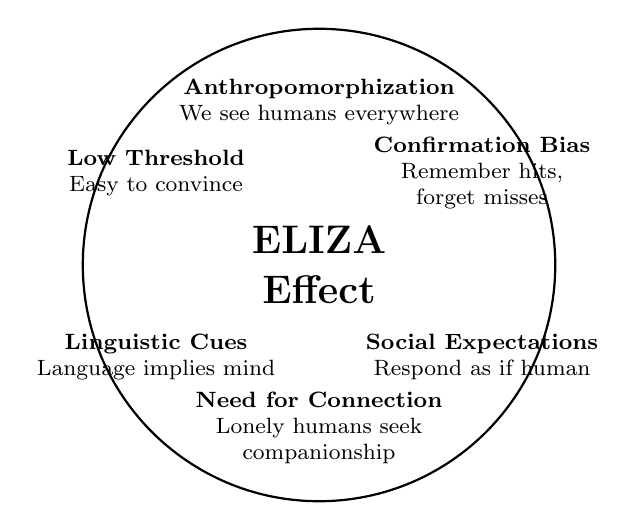
\begin{tikzpicture}[scale=0.9]
% Circle diagram showing factors
\node[circle, draw, thick, minimum size=6cm] at (0,0) {};

% Center
\node[font=\Large\bfseries, align=center] at (0,0) {ELIZA\\Effect};

% Surrounding factors
\node[align=center, font=\footnotesize] at (0,2.3) {\textbf{Anthropomorphization}\\We see humans everywhere};
\node[align=center, font=\footnotesize] at (2.3,1.3) {\textbf{Confirmation Bias}\\Remember hits,\\forget misses};
\node[align=center, font=\footnotesize] at (2.3,-1.3) {\textbf{Social Expectations}\\Respond as if human};
\node[align=center, font=\footnotesize] at (0,-2.3) {\textbf{Need for Connection}\\Lonely humans seek\\companionship};
\node[align=center, font=\footnotesize] at (-2.3,-1.3) {\textbf{Linguistic Cues}\\Language implies mind};
\node[align=center, font=\footnotesize] at (-2.3,1.3) {\textbf{Low Threshold}\\Easy to convince};

\end{tikzpicture}
\end{center}
\end{frame}

\begin{frame}[shrink=10]{Weizenbaum's Reaction 😨}
\small
\begin{alertblock}{A Shocking Discovery}
Joseph Weizenbaum was \textbf{horrified} by people's reactions to ELIZA.
\end{alertblock}

\vspace{0.3cm}

\textbf{His initial goal:}
\begin{itemize}\setlength{\itemsep}{0pt}
    \item Demonstrate the \textit{superficiality} of human-computer interaction
    \item Show that simulation $\neq$ understanding
    \item Critique overreliance on computers
\end{itemize}

\vspace{0.3cm}

\textbf{What actually happened:}
\begin{itemize}\setlength{\itemsep}{0pt}
    \item People treated ELIZA as if it understood them
    \item Some therapists wanted to use it with real patients
    \item His secretary became emotionally attached to it
    \item The opposite of what he intended!
\end{itemize}

\vspace{0.3cm}

\begin{thinkaboutit}
Weizenbaum spent the rest of his career warning about the dangers of AI!
\end{thinkaboutit}
\end{frame}

\begin{frame}{Weizenbaum's Warning ⚠️}
\small
\begin{block}{From "Computer Power and Human Reason" (1976)}
\textit{"The computer programmer is a creator of universes for which he alone is responsible. Universes of virtually unlimited complexity can be created in the form of computer programs."}
\end{block}

\vspace{0.3cm}

\textbf{His concerns:}
\begin{enumerate}\setlength{\itemsep}{0pt}
    \item People mistake \textbf{simulation for understanding}
    \item Risk of replacing \textbf{human relationships} with machines
    \item Danger of trusting AI with decisions \textbf{it doesn't understand}
    \item Questions about \textbf{what makes us human}
    \item Ethical implications of \textbf{deception} (even unintentional)
\end{enumerate}

\vspace{0.3cm}

\begin{discussion}
Are these concerns still relevant today with ChatGPT, Claude, and other modern LLMs? What has changed? What hasn't?
\end{discussion}
\end{frame}

\begin{frame}[shrink=10]{The ELIZA Effect Today 📱}
\small
\begin{block}{Modern Examples}
The ELIZA effect is alive and well:
\end{block}

\vspace{0.3cm}

\begin{itemize}\setlength{\itemsep}{0pt}
    \item 💬 People form bonds with \textbf{Replika} (AI companion app)
    \item 🤖 Users anthropomorphize \textbf{ChatGPT} and \textbf{Claude}
    \item 📞 Customers get frustrated with \textbf{chatbots} for "not understanding"
    \item 💔 Some people prefer AI therapists to human ones
    \item 🎮 Players form attachments to \textbf{NPCs} in games
    \item 🏠 People thank \textbf{Alexa} and \textbf{Siri}
\end{itemize}

\vspace{0.3cm}

\begin{thinkaboutit}
Have you ever caught yourself treating an AI as if it understands you? Why did you do it? How did it feel?
\end{thinkaboutit}
\end{frame}

\begin{frame}[shrink=5]{Simulation vs. Understanding 🎭}
\begin{center}
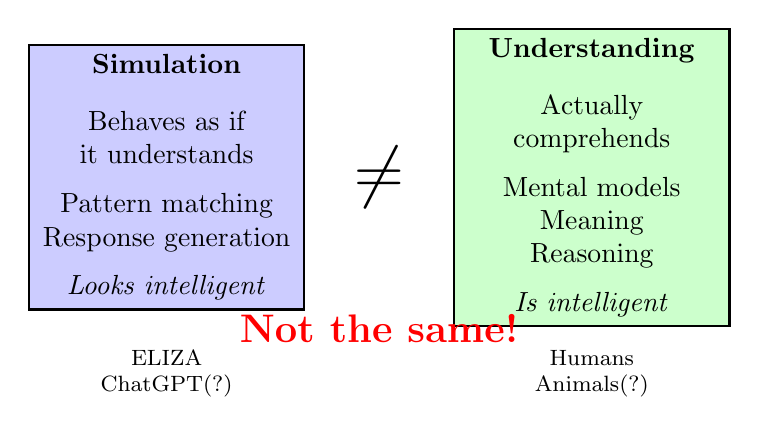
\begin{tikzpicture}[scale=0.90]
% Two boxes
\node[draw, thick, fill=blue!20, minimum width=3.5cm, minimum height=2.5cm, align=center] at (0,0) {
    \textbf{Simulation}\\[0.3cm]
    Behaves as if\\it understands\\[0.2cm]
    Pattern matching\\Response generation\\[0.2cm]
    \textit{Looks intelligent}
};

\node[draw, thick, fill=green!20, minimum width=3.5cm, minimum height=2.5cm, align=center] at (6,0) {
    \textbf{Understanding}\\[0.3cm]
    Actually\\comprehends\\[0.2cm]
    Mental models\\Meaning\\Reasoning\\[0.2cm]
    \textit{Is intelligent}
};

% Question mark between
\node[font=\Huge] at (3,0) {$\neq$};
\node[below, red, font=\Large\bfseries] at (3,-1.8) {Not the same!};

% Examples below
\node[below, font=\footnotesize, align=center] at (0,-2.3) {ELIZA\\ChatGPT(?)};
\node[below, font=\footnotesize, align=center] at (6,-2.3) {Humans\\Animals(?)};

\end{tikzpicture}
\end{center}

\begin{discussion}
Is there a clear line between simulation and understanding? Or is it a spectrum?
\end{discussion}
\end{frame}

\section{From ELIZA to Modern LLMs}

\begin{frame}[shrink=5]{The Evolution of Chatbots 📈}
\begin{center}
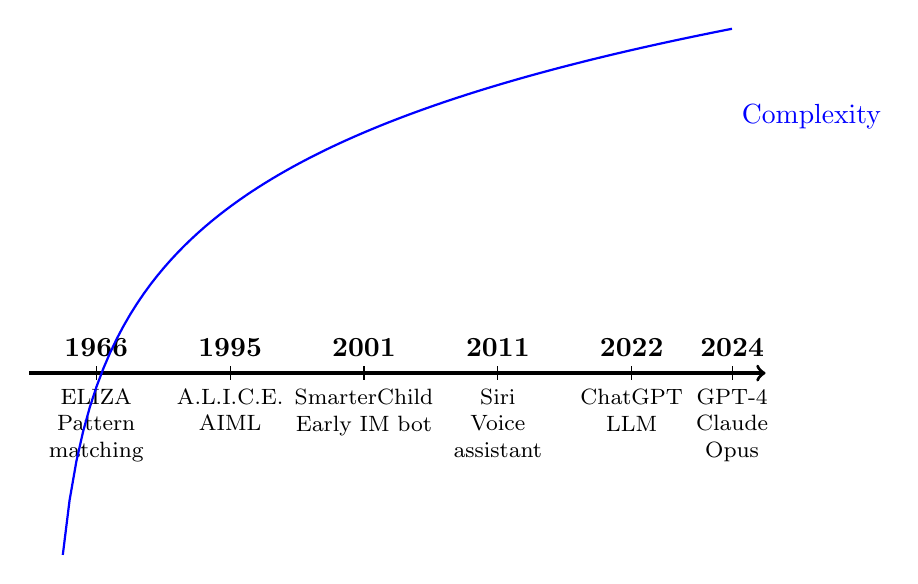
\begin{tikzpicture}[scale=0.85]
% Timeline
\draw[very thick, ->] (0,0) -- (11,0);

% Markers
\node[above] at (1,0.1) {\textbf{1966}};
\node[below, align=center, font=\footnotesize] at (1,-0.1) {ELIZA\\Pattern\\matching};

\node[above] at (3,0.1) {\textbf{1995}};
\node[below, align=center, font=\footnotesize] at (3,-0.1) {A.L.I.C.E.\\AIML};

\node[above] at (5,0.1) {\textbf{2001}};
\node[below, align=center, font=\footnotesize] at (5,-0.1) {SmarterChild\\Early IM bot};

\node[above] at (7,0.1) {\textbf{2011}};
\node[below, align=center, font=\footnotesize] at (7,-0.1) {Siri\\Voice\\assistant};

\node[above] at (9,0.1) {\textbf{2022}};
\node[below, align=center, font=\footnotesize] at (9,-0.1) {ChatGPT\\LLM};

\node[above] at (10.5,0.1) {\textbf{2024}};
\node[below, align=center, font=\footnotesize] at (10.5,-0.1) {GPT-4\\Claude\\Opus};

% Complexity curve
\draw[thick, blue, domain=0.5:10.5, samples=100]
    plot (\x, {0.5 + 2*ln(\x-0.3)});

\node[blue, above right] at (10.5,3.5) {Complexity};

% Tick marks
\foreach \x in {1,3,5,7,9,10.5} {
    \draw (\x,0.1) -- (\x,-0.1);
}
\end{tikzpicture}
\end{center}

\vspace{0.3cm}

\begin{block}{Key Point}
We've moved from hand-crafted rules to learned patterns, but the fundamental idea remains: \textbf{pattern matching at scale}.
\end{block}
\end{frame}

\begin{frame}[shrink=10]{ELIZA vs Modern LLMs: Comparison 📊}
\small
\begin{columns}
\begin{column}{0.48\textwidth}
\textbf{ELIZA (1966):}
\begin{itemize}\setlength{\itemsep}{0pt}
    \item ✍️ Hand-written rules
    \item 🔢 $\sim$200 patterns
    \item 🎯 Domain-specific (therapy)
    \item 💾 Tiny memory footprint
    \item ⚡ Instant responses
    \item 🎲 Random template selection
    \item ❌ No learning
    \item ❌ No context beyond memory
    \item ❌ Easily fooled
\end{itemize}
\end{column}

\begin{column}{0.48\textwidth}
\textbf{GPT-4 (2023):}
\begin{itemize}\setlength{\itemsep}{0pt}
    \item 🤖 Learned from data
    \item 🔢 1.7+ trillion parameters
    \item 🌍 General purpose
    \item 💾 Massive model
    \item ⏱️ Slower responses
    \item 🧮 Statistical prediction
    \item ✅ Continuous learning (training)
    \item ✅ Long context windows
    \item ❓ Harder to fool, but possible
\end{itemize}
\end{column}
\end{columns}

\vspace{0.3cm}

\begin{thinkaboutit}
GPT-4 is incomparably more sophisticated, but does it truly "understand" or is it just better pattern matching?
\end{thinkaboutit}
\end{frame}

\begin{frame}[shrink=10]{What ELIZA Teaches Us 🎓}
\small
\begin{block}{Lessons from a 60-Year-Old Program}
ELIZA remains relevant because it reveals fundamental truths:
\end{block}

\vspace{0.3cm}

\begin{enumerate}\setlength{\itemsep}{0pt}
    \item \textbf{Behavior $\neq$ Understanding}: Looking intelligent is not the same as being intelligent
    \item \textbf{Human Psychology}: We \textit{want} to believe machines understand us
    \item \textbf{Simplicity is powerful}: You don't need complexity to create illusions
    \item \textbf{Context matters}: Without it, even good patterns fail
    \item \textbf{Ethics are crucial}: Deception (even unintentional) has consequences
    \item \textbf{Building reveals truth}: Making something yourself shows its limitations
\end{enumerate}

\vspace{0.3cm}

\begin{alertblock}{Why We Study ELIZA}
By building ELIZA, you'll understand what AI \textit{really} is—and what it isn't!
\end{alertblock}
\end{frame}

\section{Assignment 1: Build Your Own ELIZA}

\begin{frame}[shrink=10]{Assignment 1: Build ELIZA 🛠️}
\small
\begin{alertblock}{Your First Assignment}
You will implement your own version of the ELIZA chatbot!
\end{alertblock}

\vspace{0.3cm}

\textbf{What you'll do:}
\begin{enumerate}\setlength{\itemsep}{0pt}
    \item Read rules from a configuration file
    \item Implement pre-substitutions
    \item Handle synonym substitutions
    \item Implement pattern matching with regex
    \item Implement decomposition and reassembly
    \item Apply post-substitutions
    \item Create a conversation loop
    \item (Optional) Add memory functionality
\end{enumerate}

\vspace{0.3cm}

\begin{thinkaboutit}
This will be challenging but incredibly rewarding! You'll truly understand how chatbots work.
\end{thinkaboutit}
\end{frame}

\begin{frame}[shrink=10]{Assignment Structure 📋}
\small
\begin{columns}
\begin{column}{0.5\textwidth}
\textbf{Technical requirements:}
\begin{itemize}\setlength{\itemsep}{0pt}
    \item Python implementation
    \item Use provided \texttt{instructions.txt}
    \item Pattern matching with regex
    \item Proper text substitutions
    \item Conversation loop
    \item Greeting \& goodbye messages
    \item At least 20 patterns
    \item Handle edge cases
\end{itemize}
\end{column}

\begin{column}{0.5\textwidth}
\textbf{Deliverable:}
\begin{itemize}\setlength{\itemsep}{0pt}
    \item Single Jupyter notebook
    \item Runnable in Google Colab
    \item Markdown explanations
    \item Example conversations
    \item Well-documented code
    \item Reflection section
    \item Discussion of limitations
\end{itemize}
\end{column}
\end{columns}

\vspace{0.3cm}

\begin{block}{Due Date}
Check Canvas for the exact due date! Usually 2 weeks from today.
\end{block}
\end{frame}

\begin{frame}[fragile]{The Configuration File Format 📄}
\textbf{Example \texttt{instructions.txt} structure:}

\begin{lstlisting}[basicstyle=\ttfamily\tiny]
# Pre-substitutions
PRE_SUB: dont -> don't
PRE_SUB: cant -> can't
PRE_SUB: wont -> won't

# Synonyms
SYNONYM: family -> family, relatives, kin, folks
SYNONYM: sad -> sad, unhappy, depressed, down, blue

# Patterns (rank, pattern, responses)
PATTERN: 100, (.*) @family (.*), Tell me more about your family.|How do you feel about your family?|What role does your family play in this?

PATTERN: 80, I am @sad, Why are you {1}?|How long have you been {1}?|What makes you {1}?

PATTERN: 50, I (.*) my (.*), Tell me more about your {2}.|How does your {2} make you feel?

PATTERN: 10, (.*), Tell me more.|I see.|How does that make you feel?

# Post-substitutions
POST_SUB:  i  ->  you
POST_SUB:  my  ->  your
POST_SUB:  am  ->  are
\end{lstlisting}
\end{frame}

\begin{frame}{Grading Rubric ✅}
\begin{center}
\begin{tabular}{lc}
\toprule
\textbf{Component} & \textbf{Points} \\
\midrule
Pre-substitutions working & 10 \\
Synonym substitutions & 10 \\
Pattern matching (regex) & 20 \\
Capture and reassembly & 15 \\
Post-substitutions & 10 \\
Conversation loop & 10 \\
Code quality \& documentation & 10 \\
Example conversations & 5 \\
Reflection \& analysis & 10 \\
\midrule
\textbf{Total} & \textbf{100} \\
\bottomrule
\end{tabular}
\end{center}

\vspace{0.3cm}

\textbf{Bonus (up to +10):}
\begin{itemize}\setlength{\itemsep}{0pt}
    \item Memory implementation (+5)
    \item Particularly creative patterns (+5)
\end{itemize}
\end{frame}

\begin{frame}[shrink=10]{Tips for Success 💡}
\begin{enumerate}\setlength{\itemsep}{0pt}
    \item \textbf{Start early!} Pattern matching can be tricky
    \item \textbf{Test incrementally}: Build one piece at a time
    \item \textbf{Use print statements}: Debug by seeing what patterns match
    \item \textbf{Read Weizenbaum (1966)}: Understand the original design
    \item \textbf{Test with edge cases}: What if input is empty? Very long?
    \item \textbf{Experiment}: Try having conversations with your bot
    \item \textbf{Use regex testers}: \href{https://regex101.com}{regex101.com} is your friend!
    \item \textbf{Collaborate}: Discuss ideas with classmates (but write your own code!)
    \item \textbf{Ask questions}: Use Discord and office hours
    \item \textbf{Have fun!}: This should be enjoyable!
\end{enumerate}
\end{frame}

\begin{frame}{Common Pitfalls to Avoid ⚠️}
\small
\begin{alertblock}{Watch Out For:}
\begin{itemize}\setlength{\itemsep}{0pt}
    \item \textbf{Escaping special regex characters}: Use \texttt{r"..."} for raw strings
    \item \textbf{Substitution order}: Pre-subs before matching, post-subs after
    \item \textbf{Greedy vs. non-greedy matching}: \texttt{(.*)} vs \texttt{(.*?)}
    \item \textbf{Case sensitivity}: Convert to lowercase or use \texttt{(?i)} flag
    \item \textbf{Spaces in substitutions}: Use \texttt{" word "} to avoid partial matches
    \item \textbf{Empty input}: Handle edge cases gracefully
    \item \textbf{Infinite loops}: Make sure your quit condition works!
    \item \textbf{Overly specific patterns}: They'll never match real input
\end{itemize}
\end{alertblock}

\vspace{0.3cm}

\begin{thinkaboutit}
Testing is your friend! Try lots of different inputs to find bugs.
\end{thinkaboutit}
\end{frame}

\begin{frame}[fragile]{Example: Testing Your Implementation 🧪}
\begin{lstlisting}[basicstyle=\ttfamily\tiny]
# Good test cases to try:
test_inputs = [
    "I am sad",                    # Basic pattern
    "I'm depressed",               # Synonym + contraction
    "i dont like my mother",       # Pre-sub, post-sub, keyword
    "MY FATHER NEVER UNDERSTOOD ME", # Case sensitivity
    "I love my family",            # Synonym
    "",                            # Empty input
    "xyz123!@#",                   # Nonsense
    "Why do you keep asking about my family?", # Meta
    "I need to go",                # Quit pattern
]

# Test each one
for user_input in test_inputs:
    response = bot.respond(user_input)
    print(f"User: {user_input}")
    print(f"ELIZA: {response}")
    print()

# Check:
# - Does each match the expected pattern?
# - Are substitutions working?
# - Do responses make sense?
# - Any crashes or errors?
\end{lstlisting}
\end{frame}

\begin{frame}[shrink=10]{Reflection Questions 💭}
\small
\textbf{Include in your notebook:}

\begin{enumerate}\setlength{\itemsep}{0pt}
    \item What was the most challenging part of the implementation?
    \item What surprised you about how ELIZA works?
    \item Did you experience the "ELIZA effect" when testing your bot?
    \item What are the main limitations you noticed?
    \item How would you improve ELIZA if you had more time?
    \item What did this teach you about modern AI systems?
    \item Do you think ELIZA "understands" anything? Why or why not?
\end{enumerate}

\vspace{0.3cm}

\begin{thinkaboutit}
The reflection is as important as the code! It shows your critical thinking about AI.
\end{thinkaboutit}
\end{frame}

\begin{frame}[shrink=10]{Extension Ideas (Optional) 🌟}
\textbf{If you want to go further:}

\begin{itemize}\setlength{\itemsep}{0pt}
    \item 🧠 \textbf{Smarter memory}: Track topics and their sentiment
    \item 🎭 \textbf{Multiple personas}: Different rule sets for different "personalities"
    \item 📊 \textbf{Conversation analysis}: Track which patterns are used most
    \item 🎨 \textbf{GUI interface}: Build a web interface with Gradio or Streamlit
    \item 🗣️ \textbf{Voice interaction}: Add speech-to-text and text-to-speech
    \item 🌐 \textbf{Multi-language}: Patterns for another language
    \item 📝 \textbf{Learning mode}: Save new patterns from conversations
    \item 🤖 \textbf{Compare with GPT}: Run same prompts through both
\end{itemize}

\vspace{0.3cm}

\begin{alertblock}{Note}
These are optional enrichment activities—not required for full credit!
\end{alertblock}
\end{frame}

\section{Looking Ahead}

\begin{frame}{What's Next? 🔮}
\small
\begin{block}{Week 2: Computational Linguistics}
We'll move beyond simple pattern matching to explore:
\begin{itemize}\setlength{\itemsep}{0pt}
    \item \textbf{Tokenization}: How to split text into meaningful units
    \item \textbf{N-grams}: Patterns across multiple words
    \item \textbf{Statistical language models}: Predicting what comes next
    \item \textbf{Part-of-speech tagging}: Understanding grammatical roles
    \item \textbf{Web scraping}: Getting real text data
\end{itemize}
\end{block}

\vspace{0.3cm}

\begin{alertblock}{The Bridge}
Week 1 showed you pattern matching by hand. Week 2 shows you how to find patterns \textit{automatically} from data!
\end{alertblock}
\end{frame}

\begin{frame}[shrink=10]{Resources for Learning 📚}
\small
\begin{block}{Essential Reading}
\begin{itemize}\setlength{\itemsep}{0pt}
    \item \textbf{Weizenbaum (1966)}: ELIZA paper - The original!
    \item \textbf{Python regex docs}: \href{https://docs.python.org/3/library/re.html}{docs.python.org/3/library/re.html}
    \item \textbf{Regex101}: \href{https://regex101.com}{regex101.com} - Test your patterns
    \item \textbf{HuggingFace NLP Course}: \href{https://huggingface.co/course}{huggingface.co/course}
\end{itemize}
\end{block}

\vspace{0.3cm}

\begin{block}{Optional Fun Stuff}
\begin{itemize}\setlength{\itemsep}{0pt}
    \item Try talking to original ELIZA: \href{https://www.masswerk.at/elizabot/}{masswerk.at/elizabot}
    \item Watch: "How ELIZA Worked" on YouTube
    \item Read: "Computer Power and Human Reason" by Weizenbaum
\end{itemize}
\end{block}
\end{frame}

\begin{frame}[shrink=10]{Key Takeaways 🔑}
\begin{enumerate}\setlength{\itemsep}{0pt}
    \item \textbf{ELIZA is simple but powerful}: Pattern matching creates convincing illusions
    \item \textbf{The ELIZA Effect is real}: We anthropomorphize machines easily
    \item \textbf{Weizenbaum was prescient}: His warnings about AI are still relevant
    \item \textbf{Building reveals truth}: Making ELIZA shows its limitations clearly
    \item \textbf{Modern AI is similar}: More sophisticated, but still pattern matching
    \item \textbf{Critical thinking is essential}: Always question what looks intelligent
    \item \textbf{This is just the start}: Each week builds toward true understanding
\end{enumerate}

\vspace{0.3cm}

\begin{alertblock}{Remember}
The goal isn't just to build ELIZA—it's to \textit{understand} what conversation, intelligence, and understanding really mean!
\end{alertblock}
\end{frame}

\begin{frame}{Final Thoughts 💡}
\begin{center}
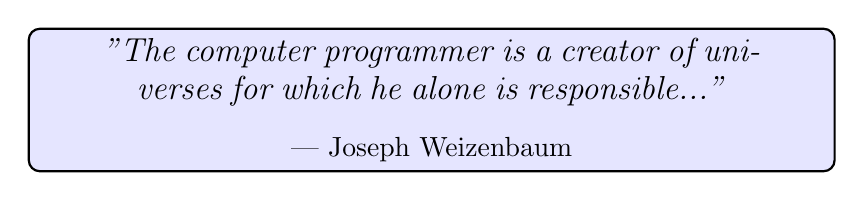
\begin{tikzpicture}[scale=0.85]
% Quote box
\node[draw, thick, fill=blue!10, rounded corners, text width=10cm, align=center] at (0,0) {
    \large\textit{"The computer programmer is a creator of universes for which he alone is responsible..."}

    \vspace{0.3cm}

    \normalsize — Joseph Weizenbaum
};
\end{tikzpicture}
\end{center}

\vspace{0.3cm}

\begin{discussion}
As you build your ELIZA, remember: You're creating a small universe. What responsibilities come with that?

How does it feel to create something that might deceive users into thinking it understands them?
\end{discussion}
\end{frame}

\begin{frame}{Questions? 🤔}
\begin{center}
\Large{Let's discuss!}

\vspace{0.5cm}

\textbf{Contact Information:}

📧 jeremy@dartmouth.edu

💬 Discord: \href{https://discord.gg/sftEk9Ygdw}{https://discord.gg/sftEk9Ygdw}

🏢 Office Hours: By appointment (Moore Hall 349)

\vspace{0.3cm}

\textbf{Assignment 1 is now available on Canvas!}

\vspace{0.3cm}

\large{Good luck building ELIZA! 🚀}
\end{center}
\end{frame}

\end{document}
